\chapter{Removing the CMS thumbprint}
\label{ch:unfolding}

The \CMS{} detector naturally smears the kinematic properties of the particles it detects, the effects of which are known as the response of the detector.
When comparing to measurements from other experiments or to simulations without the modelling of the detector, the detector response, derived from simulation, needs to be removed.
This process is known as unfolding.
There are two common approaches to the level of unfolding.
Firstly, one can unfold to parton level which extrapolates the results with respect to the constituent partons.
This has large theoretical uncertainties stemming from the modelling of the parton shower.
In addition, these measurements are usually also extrapolated to the full kinematic phase space.
The second option is to present the results to particle level, \ie{} with respect to the stable particles produced after the shower modelling where stable particles are for this purpose defined as particles with a lifetime longer than \particleLifetime{}.


\section{Particle level measurement} % (fold)
\label{sec:particle_level}

This thesis presents measurements at particle level in a phase space chosen to closely resemble that used to select events in data.
Particle-level objects are used to define the phase space which is identical for both the \eJets{} and \muJets{} channels which allows for a consistent combination after unfolding.
Particle-level objects used to define the phase space are constructed from stable particles produced in simulation by the event generator but before the detector interactions are modelled.

The generator-level descriptions of the particles are based on the \RIVET{} framework~\cite{Unfold:Rivet} following prescriptions given in~\cite{Unfold:pseudoTop}.
Simulated electrons and muons not originating from a hadron or a quark are used to define electrons and muons at particle level.  
Photons close to the lepton are assumed to have radiated from the lepton, and are clustered with it using the anti-\kt algorithm with $\DR=0.1$.  
Particle-level jets are constructed by clustering all stable particles, excluding those used in defining the leptons, with the anti-\kt algorithm with $\DR=0.4$.
If a particle-level jet originated from a \bquark{} quark, \bquark{} hadrons are included in the clustering of jets but with the magnitude of the four momenta scaled to negligible values. 
They are known as \textit{ghost} particles, because they do not affect the kinematic properties of the jet.
A jet with a constituent \bquark{} hadron is considered to have originated from a \bquark{} quark.
The particle-level \ptmiss{} is calculated from all stable visible particles.

The visible phase space is given by a single particle-level electron or muon with $\LPT>26\GeV$ and $\LETA<2.4$.
Events with additional leptons of $\LPT>15\GeV$ and $\LETA<2.4$ are not permitted.
The particle-level jet selection differs slightly from that in data.
Three particle-level jets must have $\pt>30\GeV$ and the fourth a relaxed cut of $\pt>20\GeV$.
Two of the particle-level jets need to be tagged as originating from a \bquark{} quark.
The variables \HT{}, \ST{} and \NJET{} are subsequently calculated with respect to all jets with $\pt>20\GeV$. 

As stated in Sec.~\ref{sub:calculating_the_yield}, the yield of \ttbar{} events for each bin in data is obtained by subtracting the contribution of each background process. In addition, the contribution of \ttbar events which satisfy the selection criteria, but do not enter the visible phase space at particle level, is estimated from simulation and subtracted from the data. 
This accounts for $\sim7\%$ of all \ttbar{} events and are predominately those
in which one of the jets fails the particle-level jet selection, but passes the reconstructed jet selection because of the resolution of the detector. 
The relaxed particle-level jet selection reduced this fraction from $\sim20\%$ to create the largest possible data sample.
The effect on the total uncertainty from this additional extrapolation is negligible.
No selection is applied on the decay channel of the top quarks, so the phase space does not exclusively contain single electron or muon \ttbar{} events. 
In particular, there are contributions from events where one top quark decays to a tau lepton and subsequently to an electron or muon, or where both top quarks decay leptonically but one lepton is not within the particle-level acceptance.

\section{Choice of bins} % (fold)
\label{sec:choice_of_bins}

Events can migrate between bins of the measurement because of the finite resolution of the \CMS{} detector, \ie{} the reconstructed variable can have a different value and so can be in a different bin compared to the particle-level variable.  
The choice of binning can be used to minimise migrations.
The binning scheme for each of the event variables, with the exception of the jet multiplicity whose binning is naturally defined, is created by iteratively adding together fine bins of that variable until a set of binning criteria is met.

The primary criteria to reduce the level of migration can be represented by the purity $p$ and stability $s$ of the bin which are defined as
\begin{equation*}
p^{i} = \frac{N^{i}_{\mathrm{rec\&gen}}}{N^{i}_{\mathrm{rec}}}
\end{equation*}
and
\begin{equation*}
s^{i} = \frac{N^{i}_{\mathrm{rec\&gen}}}{N^{i}_{\mathrm{gen}}},
\end{equation*}
where $N^{i}_{\mathrm{rec\&gen}}$ is the number of events generated and reconstructed in bin $i$ and $N^{i}_{\mathrm{rec}}$($N^{i}_{\mathrm{gen}}$) is the number of events reconstructed(generated) in bin $i$.  
Purity measures the effect of migrations into bins and stability migrations out of bins.
By requiring $p^{i}$ and $s^{i}>0.6$ an acceptable balance between the minimisation of the migration of events between bins and the retention of information is obtained.
% No migration in fewer bins - but less differential information
This purity and stability cuts are reduced to 0.5 for \ptmiss{}, due to its naturally low resolution.
Figure~\ref{fig:PurityStability1} shows the purity and stability of bins in the \eJets{} channel and Fig.~\ref{fig:PurityStability2} in the \muJets{} channel.
\begin{figure}[hp]
	\centering
	\includegraphics[width=0.32\textwidth]{/Users/db0268/Mount/SoolinScratch/DPS/DPSTestingGround/DailyPythonScripts/plots/binning/purity_stability/electron_NJets_purityStability.pdf}
	\includegraphics[width=0.32\textwidth]{/Users/db0268/Mount/SoolinScratch/DPS/DPSTestingGround/DailyPythonScripts/plots/binning/purity_stability/electron_HT_purityStability.pdf}
	\includegraphics[width=0.32\textwidth]{/Users/db0268/Mount/SoolinScratch/DPS/DPSTestingGround/DailyPythonScripts/plots/binning/purity_stability/electron_ST_purityStability.pdf}\\
	\includegraphics[width=0.32\textwidth]{/Users/db0268/Mount/SoolinScratch/DPS/DPSTestingGround/DailyPythonScripts/plots/binning/purity_stability/electron_MET_purityStability.pdf}
	\includegraphics[width=0.32\textwidth]{/Users/db0268/Mount/SoolinScratch/DPS/DPSTestingGround/DailyPythonScripts/plots/binning/purity_stability/electron_WPT_purityStability.pdf} \\
	\includegraphics[width=0.32\textwidth]{/Users/db0268/Mount/SoolinScratch/DPS/DPSTestingGround/DailyPythonScripts/plots/binning/purity_stability/electron_lepton_pt_purityStability.pdf}
	\includegraphics[width=0.32\textwidth]{/Users/db0268/Mount/SoolinScratch/DPS/DPSTestingGround/DailyPythonScripts/plots/binning/purity_stability/electron_abs_lepton_eta_coarse_purityStability.pdf}
	\caption[The purity and stability of the bins in the \eJets{} channel, measured using the \powhegpythia{} simulation sample.]{The purity and stability of the bins in the \eJets{} channel, measured using the \powhegpythia{} simulation sample.}
	\label{fig:PurityStability1}
\end{figure}

\begin{figure}[hp]
	\centering
	\includegraphics[width=0.32\textwidth]{/Users/db0268/Mount/SoolinScratch/DPS/DPSTestingGround/DailyPythonScripts/plots/binning/purity_stability/muon_NJets_purityStability.pdf} 
	\includegraphics[width=0.32\textwidth]{/Users/db0268/Mount/SoolinScratch/DPS/DPSTestingGround/DailyPythonScripts/plots/binning/purity_stability/muon_HT_purityStability.pdf}
	\includegraphics[width=0.32\textwidth]{/Users/db0268/Mount/SoolinScratch/DPS/DPSTestingGround/DailyPythonScripts/plots/binning/purity_stability/muon_ST_purityStability.pdf} \\
	\includegraphics[width=0.32\textwidth]{/Users/db0268/Mount/SoolinScratch/DPS/DPSTestingGround/DailyPythonScripts/plots/binning/purity_stability/muon_MET_purityStability.pdf}
	\includegraphics[width=0.32\textwidth]{/Users/db0268/Mount/SoolinScratch/DPS/DPSTestingGround/DailyPythonScripts/plots/binning/purity_stability/muon_WPT_purityStability.pdf} \\
	\includegraphics[width=0.32\textwidth]{/Users/db0268/Mount/SoolinScratch/DPS/DPSTestingGround/DailyPythonScripts/plots/binning/purity_stability/muon_lepton_pt_purityStability.pdf} 
	\includegraphics[width=0.32\textwidth]{/Users/db0268/Mount/SoolinScratch/DPS/DPSTestingGround/DailyPythonScripts/plots/binning/purity_stability/muon_abs_lepton_eta_coarse_purityStability.pdf} \\
	\caption[The purity and stability of the bins in the \muJets{} channel, measured using the \powhegpythia{} simulation sample.]{The purity and stability of the bins in the \muJets{} channel, measured using the \powhegpythia{} simulation sample.}
	\label{fig:PurityStability2}
\end{figure}



On top of purity and stability, a few other restrictions are required for the choice of binning.
The width of the bins must be at least as wide as the typical resolution of the variable in that bin. 
The resolution is calculated as the standard deviation of the distribution of the residuals $(\abs{\mathrm{Reco}-\mathrm{Gen}})$.
Figure~\ref{fig:exampleRes} shows an example of the resolution, as calculated from the one-sided residual distribution, compared to the bin width.
The left panel shows the \eJets{} channel and the right panel the \muJets{} channel for the \HT{} bin spanning $220-275\GeV$.
\begin{figure}[htpb]
	\centering
	\includegraphics[width=0.49\textwidth]{/Users/db0268/Mount/SoolinScratch/DPS/DPSTestingGround/DailyPythonScripts/plots/binning/residuals/electron_HT_1_Residual.pdf}
	\includegraphics[width=0.49\textwidth]{/Users/db0268/Mount/SoolinScratch/DPS/DPSTestingGround/DailyPythonScripts/plots/binning/residuals/muon_HT_1_Residual.pdf}
	\caption[The residual distribution for the \HT{} event variable in the eJets{} channel on the left and the \muJets{} channel on the right. The standard deviation of the half-gaussian, which is the resolution, is given as the vertical red line and compared to the bin width given as the vertical blue line.]{The residual distribution for the \HT{} event variable in the eJets{} channel on the left and the \muJets{} channel on the right. The standard deviation of the half-gaussian, which is the resolution, is given as the vertical red line and compared to the bin width given as the vertical blue line.}
	\label{fig:exampleRes}
\end{figure}
Tables~\ref{tb:binning_electron} and~\ref{tb:binning_muon} show the resolution and bin width comparisons for each bin of each variable in the \eJets{} and \muJets{} channels respectively.
% The complete set of residual distributions are shown in Appendix.TODO.

The number of reconstructed \ttbar{} events in each bin as estimated from simulation needs to be at least 500, which corresponds to a maximum statistical uncertainty of $\approx5\%$.
If the final bin contains less than 500 events it is merged with the previous bin.
This requirement is to ensure the response matrices used in the unfolding do not introduce bias based on the statistical fluctuations of simulation.
% For well reconstructed variables, a minimum bin width requirement is imposed.
% Realistically this only effects the leptonic variables and is $<0.3$ for \LETA{} and $>$

Figure~\ref{fig:finebinHT} shows an example of the fine bin mapping between the reconstructed distribution and the particle-level distribution for the \HT{} event variable in the \eJets{} channel on the left panel and \muJets{} channel on the right panel.
The best binning scheme calculated is overlaid in red.
\begin{figure}[htpb]
	\centering
	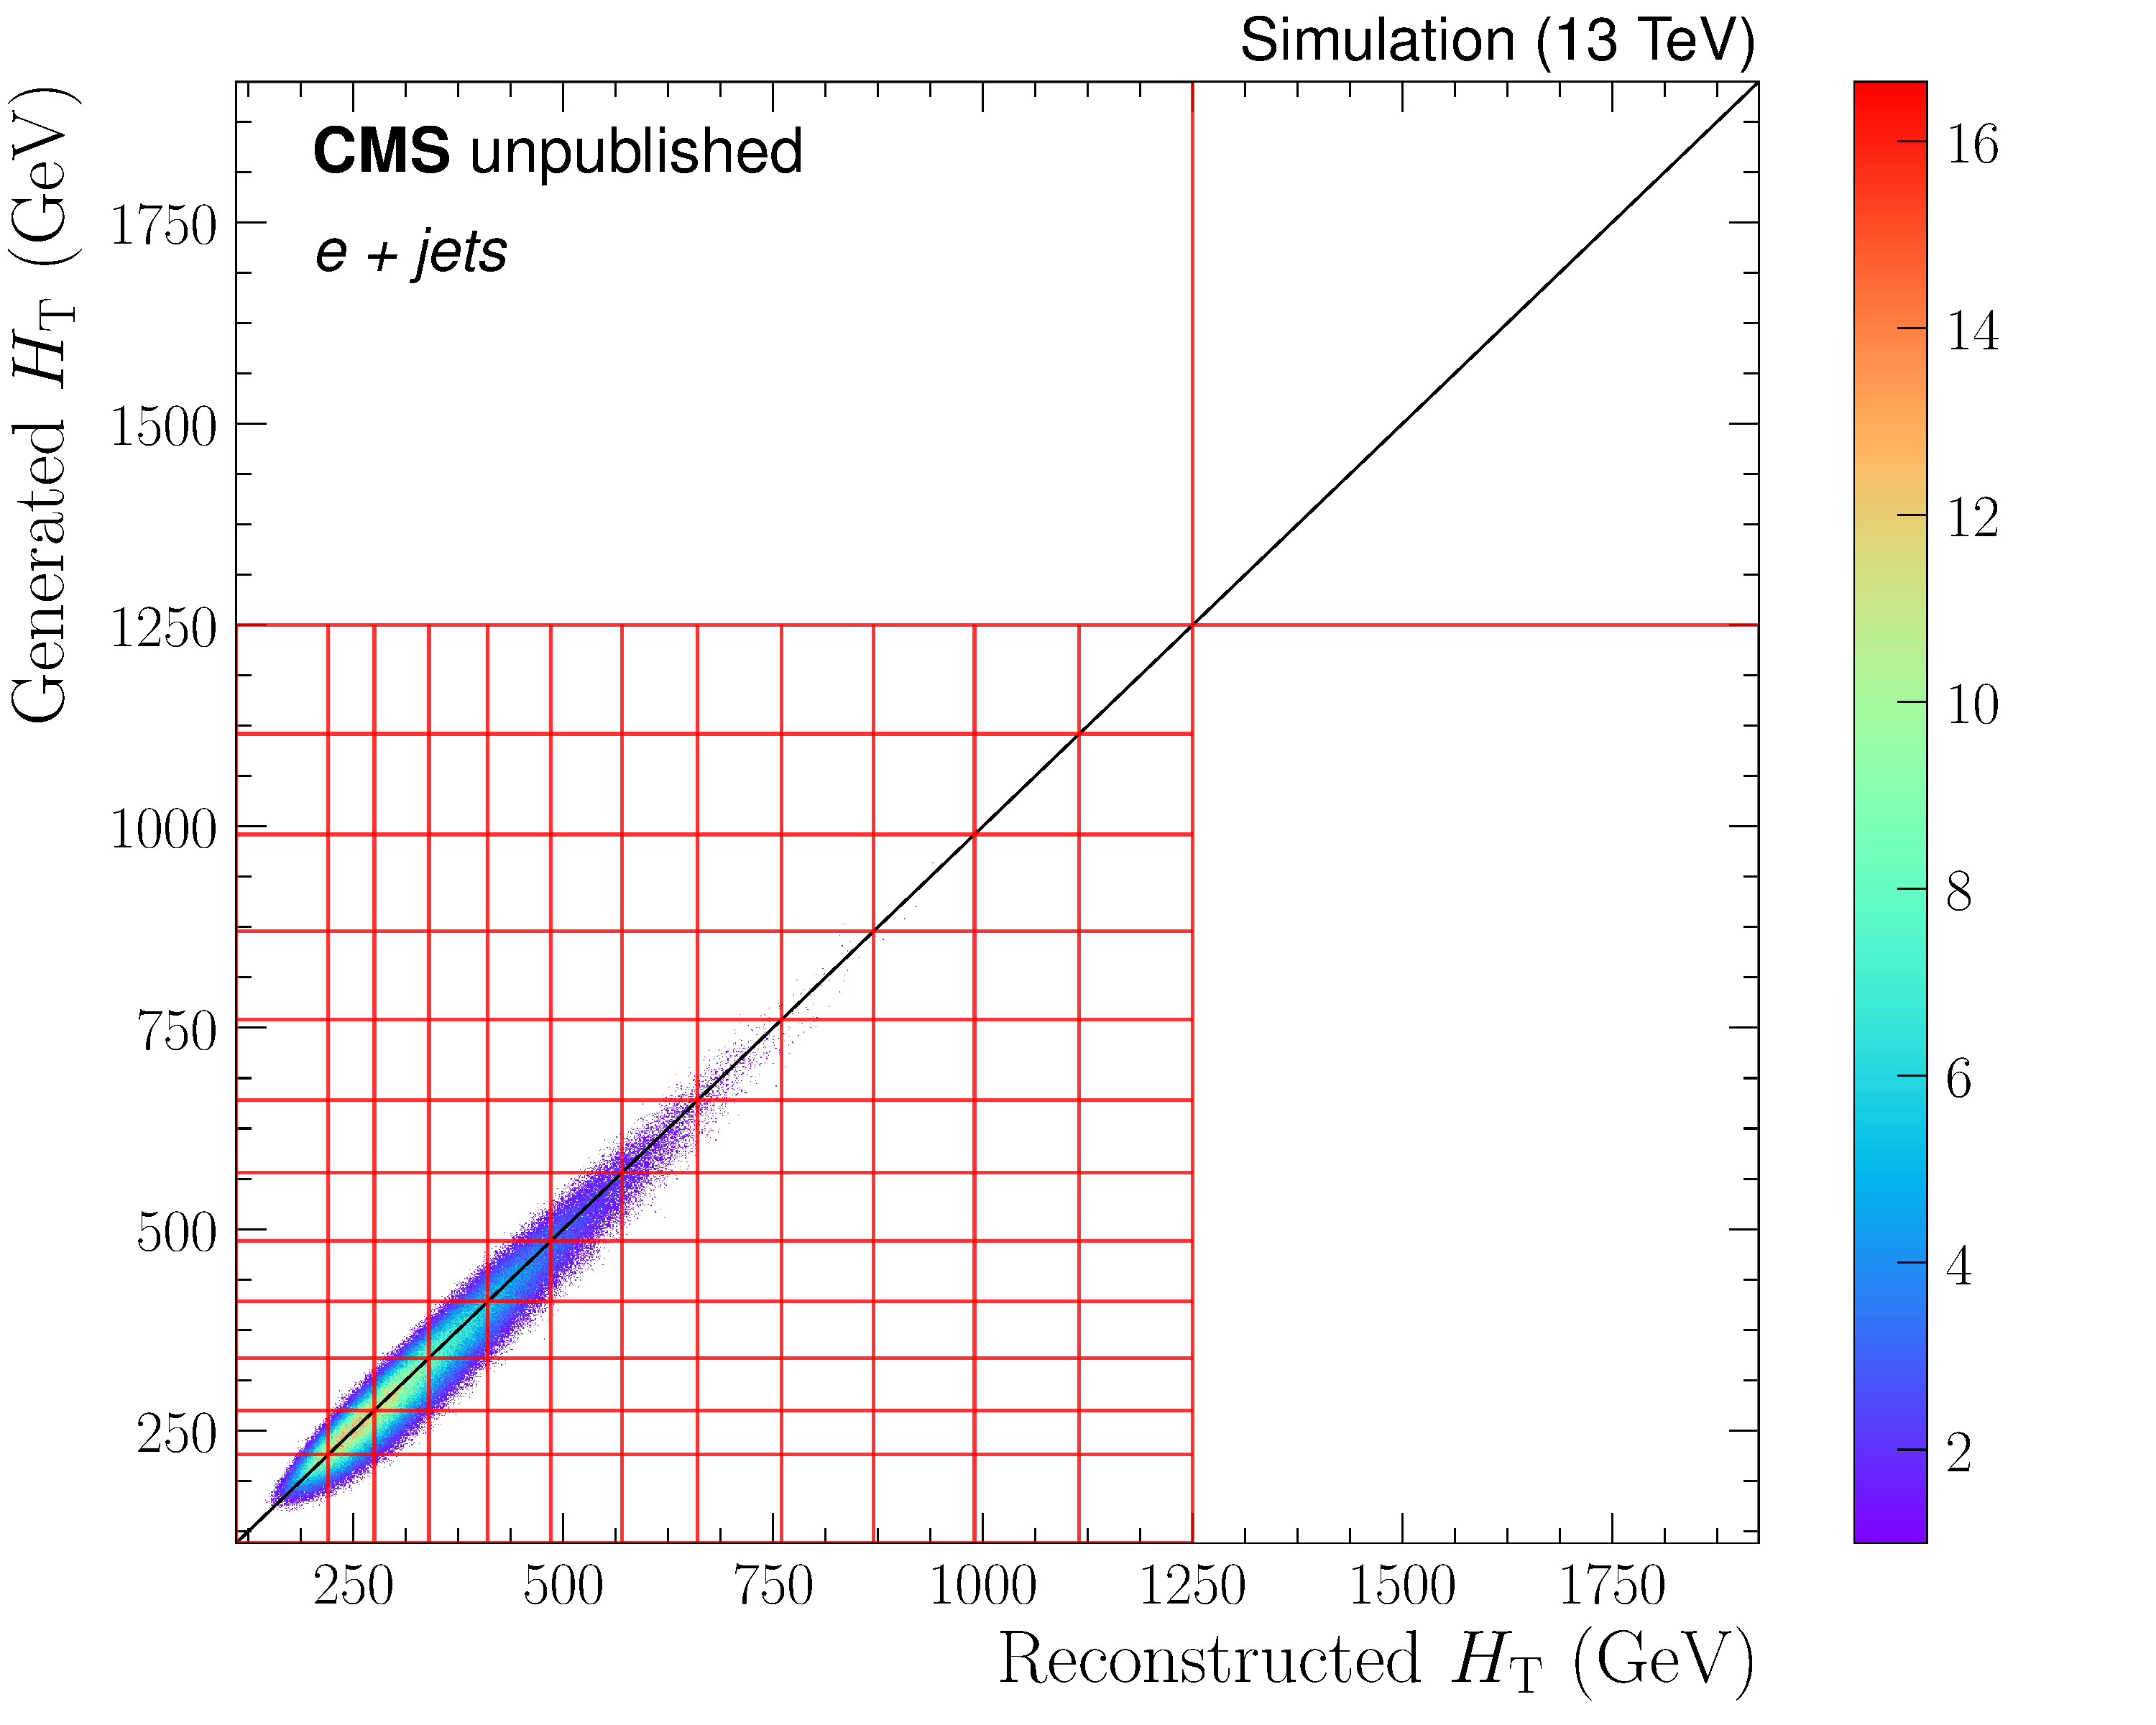
\includegraphics[width=0.49\textwidth]{Figures/electron_HT_FineBinResponse.pdf}
	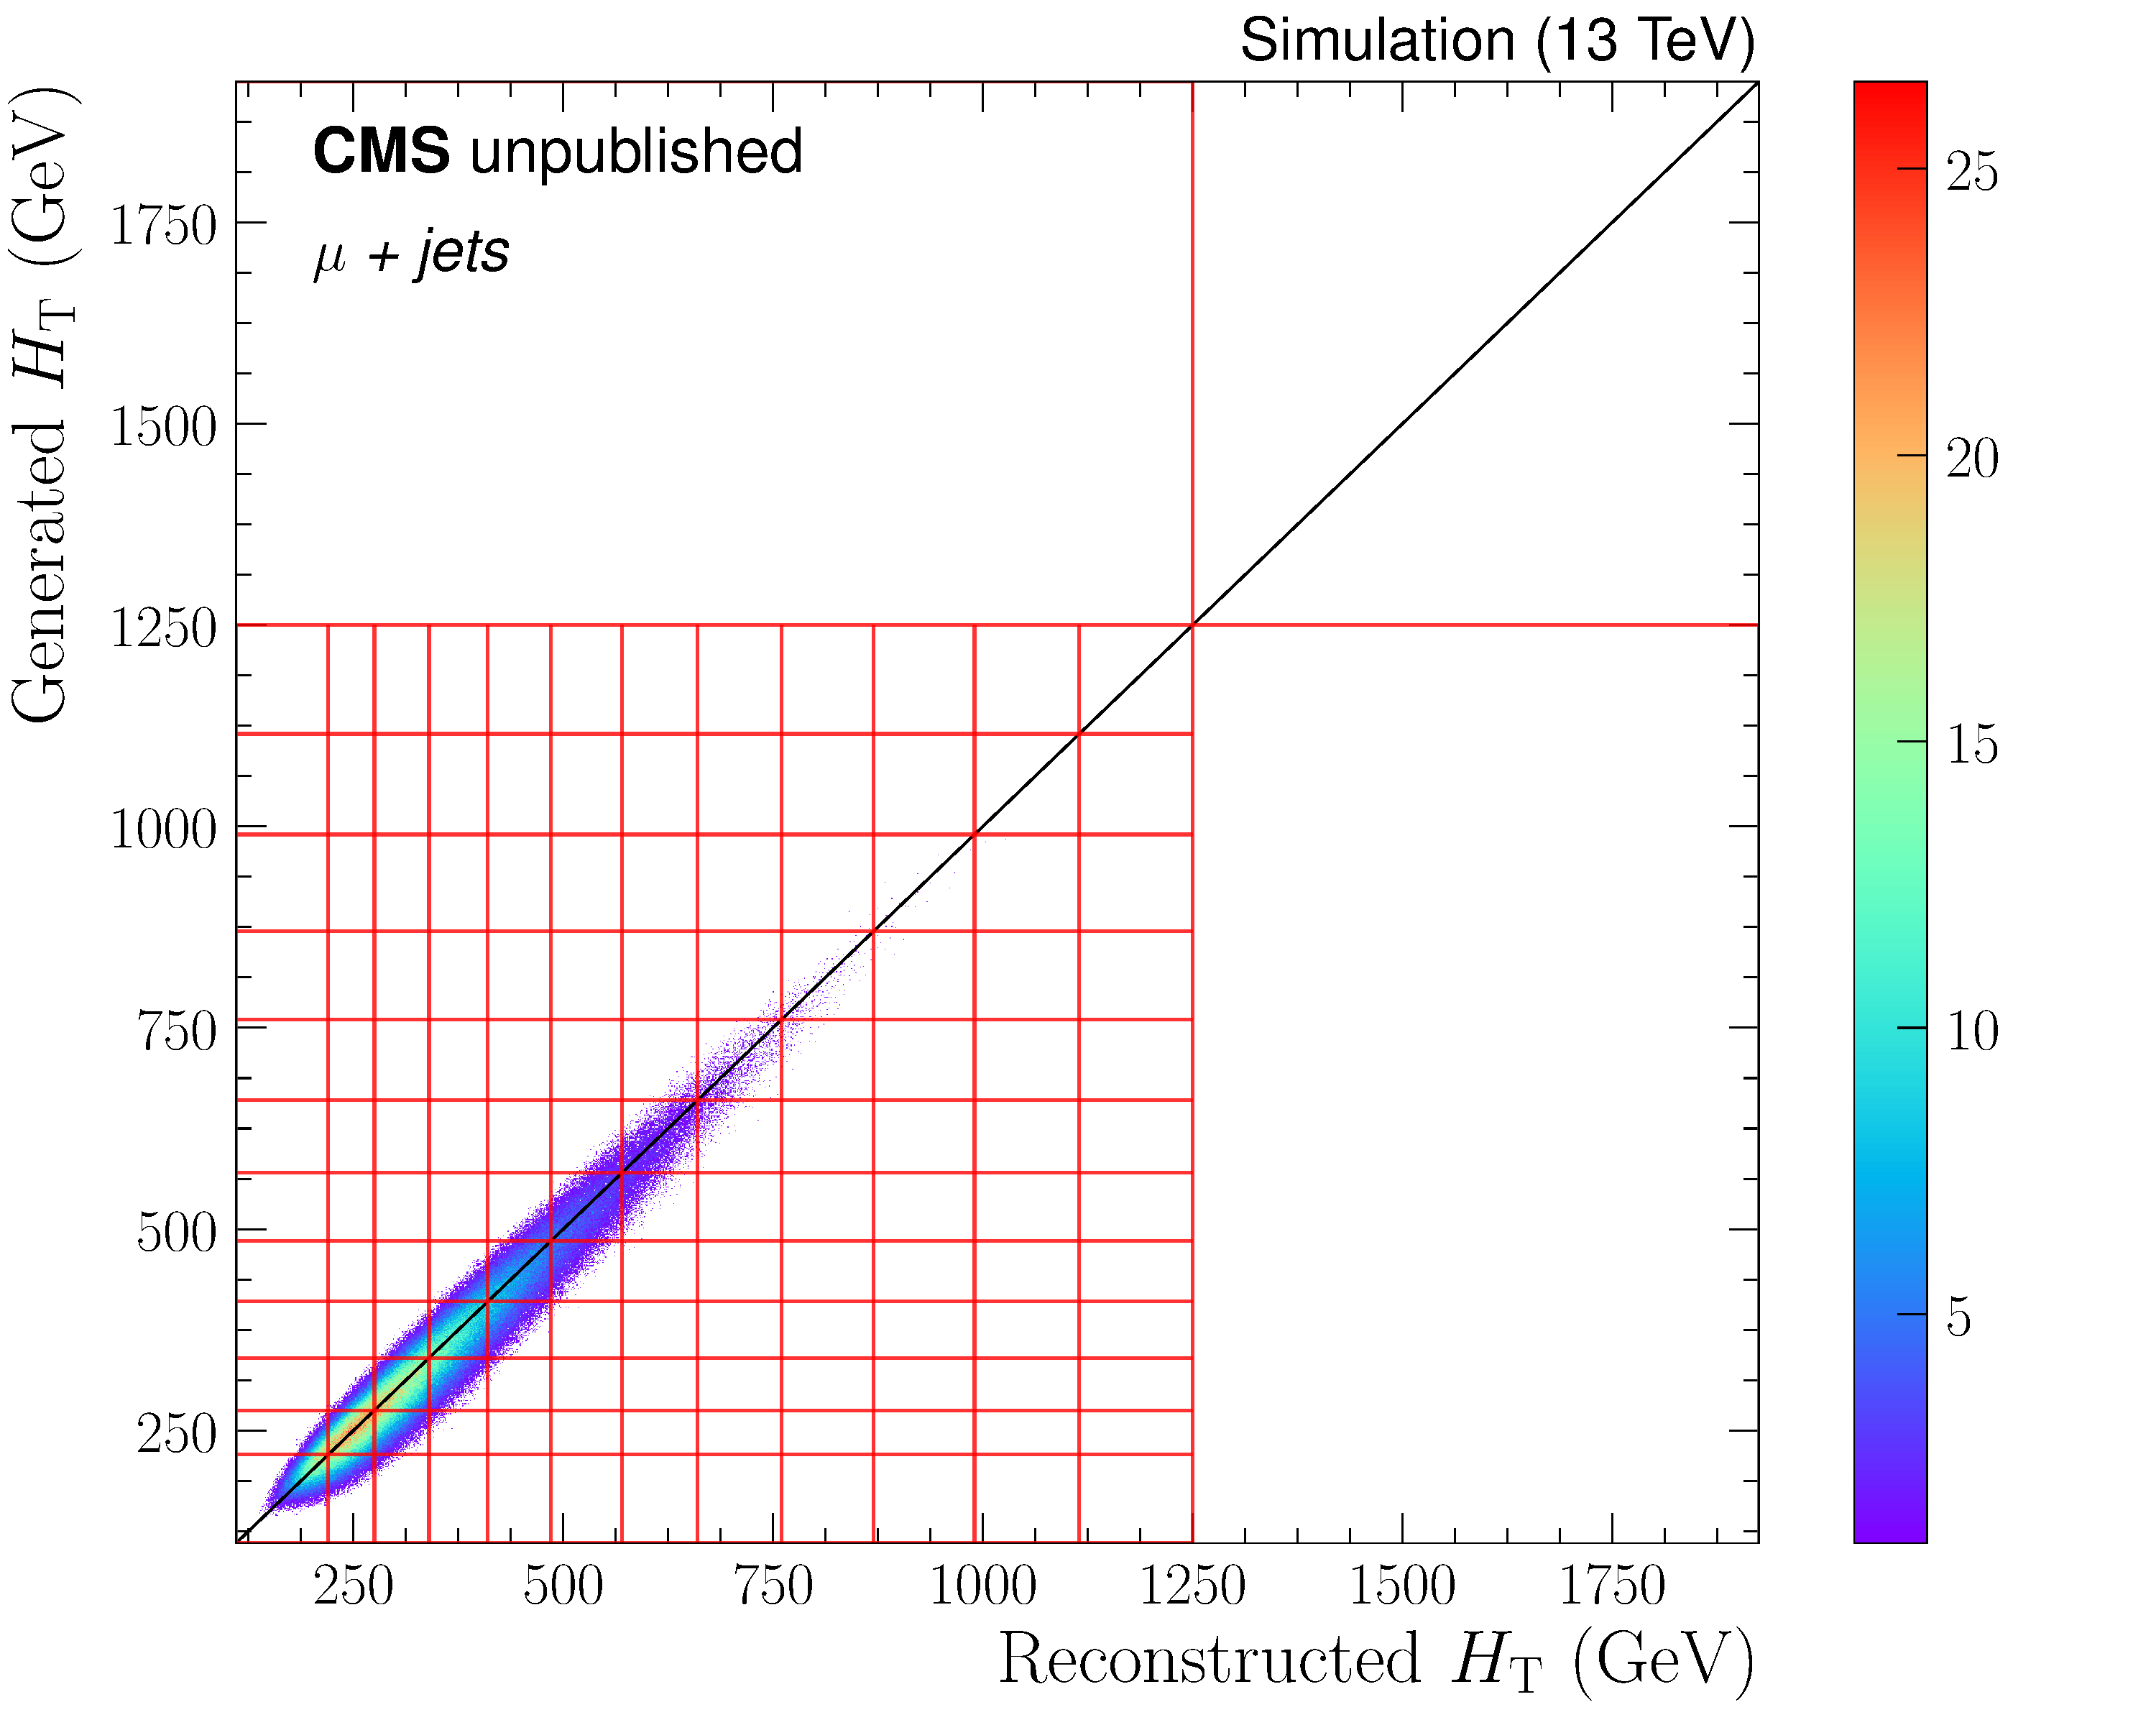
\includegraphics[width=0.49\textwidth]{Figures/muon_HT_FineBinResponse.pdf}
	\caption[The left panel shows the mapping between the reconstructed and particle-level distributions of the \HT{} event variable in the \eJets{} channel and the right panel in the \muJets{} channel. The chosen common binning scheme passing all criteria is overlaid in red.]{The left panel shows the mapping between the reconstructed and particle-level distributions of the \HT{} event variable in the \eJets{} channel and the right panel in the \muJets{} channel. The chosen common binning scheme passing all criteria is overlaid in red.}
	\label{fig:finebinHT}
\end{figure}

The response matrices for the \eJets{} and \muJets{} channels, calculated using the common binning scheme are shown in Figs.~\ref{fig:ResponseMatricesE} and~\ref{fig:ResponseMatricesMU} respectively.
The binning requirements result in a close-to-diagonal response matrix with an acceptable statistical uncertainty.

% section choice_of_bins (end)
\begin{figure}[hp]
	\centering
	\includegraphics[width=0.32\textwidth]{/Users/db0268/Mount/SoolinScratch/DPS/DPSTestingGround/DailyPythonScripts/plots/unfold_output/probability_matrices/central/NJets_electron.pdf}
	\includegraphics[width=0.32\textwidth]{/Users/db0268/Mount/SoolinScratch/DPS/DPSTestingGround/DailyPythonScripts/plots/unfold_output/probability_matrices/central/HT_electron.pdf}
	\includegraphics[width=0.32\textwidth]{/Users/db0268/Mount/SoolinScratch/DPS/DPSTestingGround/DailyPythonScripts/plots/unfold_output/probability_matrices/central/ST_electron.pdf}\\
	\includegraphics[width=0.32\textwidth]{/Users/db0268/Mount/SoolinScratch/DPS/DPSTestingGround/DailyPythonScripts/plots/unfold_output/probability_matrices/central/MET_electron.pdf}
	\includegraphics[width=0.32\textwidth]{/Users/db0268/Mount/SoolinScratch/DPS/DPSTestingGround/DailyPythonScripts/plots/unfold_output/probability_matrices/central/WPT_electron.pdf} \\
	\includegraphics[width=0.32\textwidth]{/Users/db0268/Mount/SoolinScratch/DPS/DPSTestingGround/DailyPythonScripts/plots/unfold_output/probability_matrices/central/lepton_pt_electron.pdf}
	\includegraphics[width=0.32\textwidth]{/Users/db0268/Mount/SoolinScratch/DPS/DPSTestingGround/DailyPythonScripts/plots/unfold_output/probability_matrices/central/abs_lepton_eta_coarse_electron.pdf}
	\caption[The set of response matrices, calculated using the \powhegpythia{} simulation sample and normalised to one for all event variables in the \eJets{} channel using the common binning scheme.]{The set of response matrices, calculated using the \powhegpythia{} simulation sample and normalised to one for all event variables in the \eJets{} channel using the common binning scheme.}
	\label{fig:ResponseMatricesE}
\end{figure}

\begin{figure}[hp]
	\centering
	\includegraphics[width=0.32\textwidth]{/Users/db0268/Mount/SoolinScratch/DPS/DPSTestingGround/DailyPythonScripts/plots/unfold_output/probability_matrices/central/NJets_muon.pdf} 
	\includegraphics[width=0.32\textwidth]{/Users/db0268/Mount/SoolinScratch/DPS/DPSTestingGround/DailyPythonScripts/plots/unfold_output/probability_matrices/central/HT_muon.pdf}
	\includegraphics[width=0.32\textwidth]{/Users/db0268/Mount/SoolinScratch/DPS/DPSTestingGround/DailyPythonScripts/plots/unfold_output/probability_matrices/central/ST_muon.pdf} \\
	\includegraphics[width=0.32\textwidth]{/Users/db0268/Mount/SoolinScratch/DPS/DPSTestingGround/DailyPythonScripts/plots/unfold_output/probability_matrices/central/MET_muon.pdf}
	\includegraphics[width=0.32\textwidth]{/Users/db0268/Mount/SoolinScratch/DPS/DPSTestingGround/DailyPythonScripts/plots/unfold_output/probability_matrices/central/WPT_muon.pdf} \\
	\includegraphics[width=0.32\textwidth]{/Users/db0268/Mount/SoolinScratch/DPS/DPSTestingGround/DailyPythonScripts/plots/unfold_output/probability_matrices/central/lepton_pt_muon.pdf} 
	\includegraphics[width=0.32\textwidth]{/Users/db0268/Mount/SoolinScratch/DPS/DPSTestingGround/DailyPythonScripts/plots/unfold_output/probability_matrices/central/abs_lepton_eta_coarse_muon.pdf} \\
	\caption[The set of response matrices, calculated using the \powhegpythia{} simulation sample and normalised to one for all event variables in the \muJets{} channel using the common binning scheme.]{The set of response matrices, calculated using the \powhegpythia{} simulation sample and normalised to one for all event variables in the \muJets{} channel using the common binning scheme.}
	\label{fig:ResponseMatricesMU}
\end{figure}

\begin{landscape}
\begin{table}
	\centering
	\caption{A comparison of the bin width and the resolution in each bin for all event variables in the electon channel. }
	\label{tb:binning_electron}
	\resizebox{\linewidth}{!}{%	
	\begin{tabular}{ccc:ccc:ccc:ccc:ccc:ccc:ccc}
	\multicolumn{3}{c:}{\NJET{}} & \multicolumn{3}{c:}{\HT{}} & \multicolumn{3}{c:}{\ST{}} & \multicolumn{3}{c:}{\ptmiss{}} & \multicolumn{3}{c:}{\WPT{}} & \multicolumn{3}{c:}{\LPT{}} & \multicolumn{3}{c}{\LETA{}} \\
	Bin width & Resolution & $\frac{\mathrm{Resolution}}{\mathrm{Bin\,width}}$ & Bin width & Resolution & $\frac{\mathrm{Resolution}}{\mathrm{Bin\,width}}$ & Bin width & Resolution & $\frac{\mathrm{Resolution}}{\mathrm{Bin\,width}}$ & Bin width & Resolution & $\frac{\mathrm{Resolution}}{\mathrm{Bin\,width}}$ & Bin width & Resolution & $\frac{\mathrm{Resolution}}{\mathrm{Bin\,width}}$ & Bin width & Resolution & $\frac{\mathrm{Resolution}}{\mathrm{Bin\,width}}$ & Bin width & Resolution & $\frac{\mathrm{Resolution}}{\mathrm{Bin\,width}}$ 
	\vspace*{0.03cm} \\
	\hline
	1.0 & 1.0 & 1.0 & 110.0 & 26.4 & 0.2 & 179.0 & 33.4 & 0.2 & 50.0 & 17.1 & 0.3 & 50.0 & 21.0 & 0.4 & 14.0 & 0.9 & $<$ 0.1 & 0.30 & $<$ 0.1 & $<$ 0.1  \\ 
	1.0 & 1.0 & 1.0 & 55.0 & 27.1 & 0.5 & 75.0 & 34.2 & 0.5 & 55.0 & 28.5 & 0.5 & 55.0 & 22.6 & 0.4 & 15.0 & 1.1 & $<$ 0.1 & 0.30 & $<$ 0.1 & $<$ 0.1  \\ 
	1.0 & 1.0 & 1.0 & 65.0 & 29.4 & 0.5 & 85.0 & 38.4 & 0.5 & 70.0 & 32.0 & 0.5 & 60.0 & 26.4 & 0.4 & 15.0 & 1.3 & $<$ 0.1 & 0.30 & $<$ 0.1 & $<$ 0.1  \\ 
	1.0 & 1.0 & 1.0 & 70.0 & 31.3 & 0.4 & 90.0 & 41.9 & 0.5 & 70.0 & 32.5 & 0.5 & 75.0 & 30.2 & 0.4 & 15.0 & 1.4 & $<$ 0.1 & 0.30 & $<$ 0.1 & $<$ 0.1  \\ 
	1.0 & 1.0 & 1.0 & 75.0 & 33.8 & 0.5 & 100.0 & 45.2 & 0.5 & 70.0 & 33.8 & 0.5 & 85.0 & 33.6 & 0.4 & 15.0 & 1.6 & 0.1 & 0.30 & $<$ 0.1 & $<$ 0.1  \\ 
	2.0 & 1.0 & 0.5 & 85.0 & 36.0 & 0.4 & 105.0 & 48.8 & 0.5 & 250.0 & 34.3 & 0.1 & 90.0 & 36.6 & 0.4 & 15.0 & 1.8 & 0.1 & 0.30 & $<$ 0.1 & $<$ 0.1  \\ 
	\NA{} & \NA{} & \NA{} & 90.0 & 38.5 & 0.4 & 115.0 & 52.1 & 0.5 & \NA{} & \NA{} & \NA{} & 430.0 & 39.7 & $<$ 0.1 & 15.0 & 1.9 & 0.1 & 0.20 & $<$ 0.1 & $<$ 0.1  \\ 
	\NA{} & \NA{} & \NA{} & 100.0 & 41.1 & 0.4 & 125.0 & 56.2 & 0.4 & \NA{} & \NA{} & \NA{} & \NA{} & \NA{} & \NA{} & 15.0 & 2.1 & 0.1 & 0.40 & $<$ 0.1 & $<$ 0.1  \\ 
	\NA{} & \NA{} & \NA{} & 110.0 & 43.7 & 0.4 & 130.0 & 60.0 & 0.5 & \NA{} & \NA{} & \NA{} & \NA{} & \NA{} & \NA{} & 15.0 & 2.4 & 0.2 & \NA{} & \NA{} & \NA{}  \\ 
	\NA{} & \NA{} & \NA{} & 120.0 & 47.0 & 0.4 & 145.0 & 63.6 & 0.4 & \NA{} & \NA{} & \NA{} & \NA{} & \NA{} & \NA{} & 15.0 & 2.5 & 0.2 & \NA{} & \NA{} & \NA{}  \\ 
	\NA{} & \NA{} & \NA{} & 125.0 & 50.0 & 0.4 & 155.0 & 68.9 & 0.4 & \NA{} & \NA{} & \NA{} & \NA{} & \NA{} & \NA{} & 15.0 & 2.7 & 0.2 & \NA{} & \NA{} & \NA{}  \\ 
	\NA{} & \NA{} & \NA{} & 135.0 & 52.8 & 0.4 & 175.0 & 73.2 & 0.4 & \NA{} & \NA{} & \NA{} & \NA{} & \NA{} & \NA{} & 15.0 & 2.9 & 0.2 & \NA{} & \NA{} & \NA{}  \\ 
	\NA{} & \NA{} & \NA{} & 675.0 & 58.0 & $<$ 0.1 & 875.0 & 80.7 & $<$ 0.1 & \NA{} & \NA{} & \NA{} & \NA{} & \NA{} & \NA{} & 15.0 & 3.1 & 0.2 & \NA{} & \NA{} & \NA{}  \\ 
	\NA{} & \NA{} & \NA{} & \NA{} & \NA{} & \NA{} & \NA{} & \NA{} & \NA{} & \NA{} & \NA{} & \NA{} & \NA{} & \NA{} & \NA{} & 15.0 & 3.3 & 0.2 & \NA{} & \NA{} & \NA{}  \\ 
	\NA{} & \NA{} & \NA{} & \NA{} & \NA{} & \NA{} & \NA{} & \NA{} & \NA{} & \NA{} & \NA{} & \NA{} & \NA{} & \NA{} & \NA{} & 20.0 & 3.5 & 0.2 & \NA{} & \NA{} & \NA{}  \\ 
	\NA{} & \NA{} & \NA{} & \NA{} & \NA{} & \NA{} & \NA{} & \NA{} & \NA{} & \NA{} & \NA{} & \NA{} & \NA{} & \NA{} & \NA{} & 30.0 & 3.8 & 0.1 & \NA{} & \NA{} & \NA{}  \\ 
	\NA{} & \NA{} & \NA{} & \NA{} & \NA{} & \NA{} & \NA{} & \NA{} & \NA{} & \NA{} & \NA{} & \NA{} & \NA{} & \NA{} & \NA{} & 150.0 & 4.6 & $<$ 0.1 & \NA{} & \NA{} & \NA{}  \\ 
	\end{tabular}%
}
\end{table}
\begin{table}
	\centering
	\caption{A comparison of the bin width and the resolution in each bin for all event variables in the muon channel. }
	\label{tb:binning_muon}
	\resizebox{\linewidth}{!}{%
	\begin{tabular}{ccc:ccc:ccc:ccc:ccc:ccc:ccc}
	\multicolumn{3}{c:}{\NJET{}} & \multicolumn{3}{c:}{\HT{}} & \multicolumn{3}{c:}{\ST{}} & \multicolumn{3}{c:}{\ptmiss{}} & \multicolumn{3}{c:}{\WPT{}} & \multicolumn{3}{c:}{\LPT{}} & \multicolumn{3}{c}{\LETA{}} \\
	Bin width & Resolution & $\frac{\mathrm{Resolution}}{\mathrm{Bin\,width}}$ & Bin width & Resolution & $\frac{\mathrm{Resolution}}{\mathrm{Bin\,width}}$ & Bin width & Resolution & $\frac{\mathrm{Resolution}}{\mathrm{Bin\,width}}$ & Bin width & Resolution & $\frac{\mathrm{Resolution}}{\mathrm{Bin\,width}}$ & Bin width & Resolution & $\frac{\mathrm{Resolution}}{\mathrm{Bin\,width}}$ & Bin width & Resolution & $\frac{\mathrm{Resolution}}{\mathrm{Bin\,width}}$ & Bin width & Resolution & $\frac{\mathrm{Resolution}}{\mathrm{Bin\,width}}$ 
	\vspace*{0.03cm} \\
	\hline
	1.0 & 1.0 & 1.0 & 110.0 & 26.3 & 0.2 & 179.0 & 33.6 & 0.2 & 50.0 & 17.3 & 0.3 & 50.0 & 19.8 & 0.4 & 14.0 & 0.5 & $<$ 0.1 & 0.30 & $<$ 0.1 & $<$ 0.1  \\ 
	1.0 & 1.0 & 1.0 & 55.0 & 26.9 & 0.5 & 75.0 & 34.4 & 0.5 & 55.0 & 27.4 & 0.5 & 55.0 & 23.3 & 0.4 & 15.0 & 0.8 & $<$ 0.1 & 0.30 & $<$ 0.1 & $<$ 0.1  \\ 
	1.0 & 1.0 & 1.0 & 65.0 & 29.2 & 0.4 & 85.0 & 38.8 & 0.5 & 70.0 & 32.3 & 0.5 & 60.0 & 27.2 & 0.5 & 15.0 & 1.0 & $<$ 0.1 & 0.30 & $<$ 0.1 & $<$ 0.1  \\ 
	1.0 & 1.0 & 1.0 & 70.0 & 31.5 & 0.4 & 90.0 & 42.2 & 0.5 & 70.0 & 33.0 & 0.5 & 75.0 & 30.8 & 0.4 & 15.0 & 1.4 & $<$ 0.1 & 0.30 & $<$ 0.1 & $<$ 0.1  \\ 
	1.0 & 1.0 & 1.0 & 75.0 & 33.6 & 0.4 & 100.0 & 45.5 & 0.5 & 70.0 & 33.6 & 0.5 & 85.0 & 33.9 & 0.4 & 15.0 & 1.8 & 0.1 & 0.30 & $<$ 0.1 & $<$ 0.1  \\ 
	2.0 & 1.0 & 0.5 & 85.0 & 35.9 & 0.4 & 105.0 & 48.6 & 0.5 & 250.0 & 34.8 & 0.1 & 90.0 & 36.4 & 0.4 & 15.0 & 2.2 & 0.1 & 0.30 & $<$ 0.1 & $<$ 0.1  \\ 
	\NA{} & \NA{} & \NA{} & 90.0 & 38.2 & 0.4 & 115.0 & 52.4 & 0.5 & \NA{} & \NA{} & \NA{} & 430.0 & 39.7 & $<$ 0.1 & 15.0 & 2.7 & 0.2 & 0.20 & $<$ 0.1 & $<$ 0.1  \\ 
	\NA{} & \NA{} & \NA{} & 100.0 & 40.9 & 0.4 & 125.0 & 56.1 & 0.4 & \NA{} & \NA{} & \NA{} & \NA{} & \NA{} & \NA{} & 15.0 & 3.3 & 0.2 & 0.40 & $<$ 0.1 & $<$ 0.1  \\ 
	\NA{} & \NA{} & \NA{} & 110.0 & 43.6 & 0.4 & 130.0 & 59.4 & 0.5 & \NA{} & \NA{} & \NA{} & \NA{} & \NA{} & \NA{} & 15.0 & 3.9 & 0.3 & \NA{} & \NA{} & \NA{}  \\ 
	\NA{} & \NA{} & \NA{} & 120.0 & 46.4 & 0.4 & 145.0 & 63.9 & 0.4 & \NA{} & \NA{} & \NA{} & \NA{} & \NA{} & \NA{} & 15.0 & 4.6 & 0.3 & \NA{} & \NA{} & \NA{}  \\ 
	\NA{} & \NA{} & \NA{} & 125.0 & 49.0 & 0.4 & 155.0 & 68.8 & 0.4 & \NA{} & \NA{} & \NA{} & \NA{} & \NA{} & \NA{} & 15.0 & 5.3 & 0.4 & \NA{} & \NA{} & \NA{}  \\ 
	\NA{} & \NA{} & \NA{} & 135.0 & 52.5 & 0.4 & 175.0 & 72.7 & 0.4 & \NA{} & \NA{} & \NA{} & \NA{} & \NA{} & \NA{} & 15.0 & 5.9 & 0.4 & \NA{} & \NA{} & \NA{}  \\ 
	\NA{} & \NA{} & \NA{} & 675.0 & 58.8 & $<$ 0.1 & 875.0 & 82.0 & $<$ 0.1 & \NA{} & \NA{} & \NA{} & \NA{} & \NA{} & \NA{} & 15.0 & 6.0 & 0.4 & \NA{} & \NA{} & \NA{}  \\ 
	\NA{} & \NA{} & \NA{} & \NA{} & \NA{} & \NA{} & \NA{} & \NA{} & \NA{} & \NA{} & \NA{} & \NA{} & \NA{} & \NA{} & \NA{} & 15.0 & 6.5 & 0.4 & \NA{} & \NA{} & \NA{}  \\ 
	\NA{} & \NA{} & \NA{} & \NA{} & \NA{} & \NA{} & \NA{} & \NA{} & \NA{} & \NA{} & \NA{} & \NA{} & \NA{} & \NA{} & \NA{} & 20.0 & 7.5 & 0.4 & \NA{} & \NA{} & \NA{}  \\ 
	\NA{} & \NA{} & \NA{} & \NA{} & \NA{} & \NA{} & \NA{} & \NA{} & \NA{} & \NA{} & \NA{} & \NA{} & \NA{} & \NA{} & \NA{} & 30.0 & 8.6 & 0.3 & \NA{} & \NA{} & \NA{}  \\ 
	\NA{} & \NA{} & \NA{} & \NA{} & \NA{} & \NA{} & \NA{} & \NA{} & \NA{} & \NA{} & \NA{} & \NA{} & \NA{} & \NA{} & \NA{} & 150.0 & 11.3 & $<$ 0.1 & \NA{} & \NA{} & \NA{}  \\ 
	\end{tabular}%
}
\end{table}
\end{landscape}


% \input{Plots/Plots_Binning.tex}
% \input{Plots/Plots_Res.tex}

\section{Unfolding} % (fold)
\label{sec:unfolding}

The unfolding is performed using the TUnfold algorithm~\cite{Unfold:TUnfold}. 
A schematic of the unfolding process is shown in Fig.~\ref{fig:migration}.
It shows the relation between the true distribution $\vec{x}$ and the measured distribution $\vec{y}$.
The matrix of probabilities $\mathbf{A}$ describes the migrations from a bin of the true distribution into any of the reconstructed bins.
The average expected count of events $\overtilde{y}$ differs from the observed event counts due to statistical fluctuations.
\begin{figure}[htpb]
	\centering
	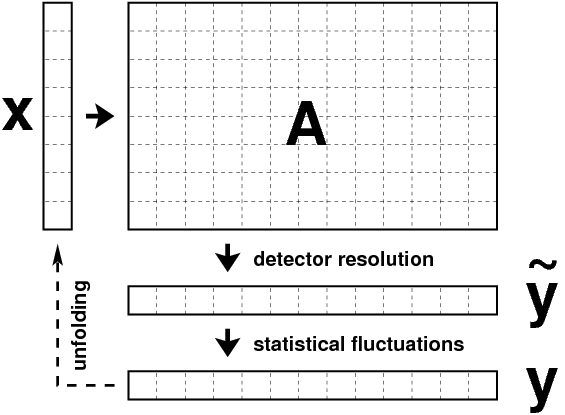
\includegraphics[width=0.65\textwidth]{Figures/Unfold_TUnfold.png}
	\caption[A schematic view of the migration effects and statistical fluctuations.]{A schematic view of the migration effects and statistical fluctuations. Figure taken from~\cite{Unfold:TUnfold}.}
	\label{fig:migration}
\end{figure}

The TUnfold algorithm uses a least squares method of estimating the true distribution $\vec{x}$ from the reconstructed distribution $\vec{y}$.
Statistical fluctuations are smoothed using Tikhonov regularisation. 
The algorithm works to minimise 
\begin{equation*}
\Lagr(x) = \Lagr_{1}+\Lagr_{2}
\end{equation*}
by finding the stationary point, where
\begin{equation*}
\Lagr_{1} = (\vec{y}-\mathbf{A}\vec{x})^{\mathrm{T}} \mathbf{V}_{yy}^{-1} (\vec{y}-\mathbf{A}\vec{x})
\end{equation*}
and
\begin{equation*}
\Lagr_{2} = \tau^{2}(\vec{x}-f_{b}\vec{x}_{0})^{\mathrm{T}} (\mathbf{L}^{\mathrm{T}}\mathbf{L}) (\vec{x}-f_{b}\vec{x}_{0}).
\end{equation*}

$\Lagr_{1}$ represents the least squares minimisation and $\Lagr_{2}$ describes the regularisation. 
$\Lagr_{1}$ involves the measured observable distribution $\vec{y}$ composed of $m$ bins and the inverse of its covariance matrix $\mathbf{V}_{yy}^{-1}$.
The covariance matrix is diagonal and holds the square of the statistical uncertainty. 
The response matrix $\mathbf{A}$ is derived from the simulated \powhegpythia{} sample.

$\Lagr_{2}$ damps fluctuations in $\vec{x}$ stemming from statistical fluctuations in $\vec{y}$. 
The parameter $\tau^2$ defines the strength of the regularisation.
If it is too small then the unfolding often yields results with large fluctuations leading to large negative correlations between neighbouring bins.
If it is too large then the result will be biased towards the input model $\vec{x}_{0}$.
The parameter $f_{b}$ decides whether to use a bias distribution based on a model ($f_{b} = 1$), suppressing differences between unfolded data and model, or to suppress the differences between the unfolded data and 0 ($f_{b} = 0$). 
This thesis sets $f_{b}=1$.
Regularisation can be done by suppressing the differences between either the size, the derivative or the curvature (second derivative) of the unfolded distribution. 
These are given by the choice of $\mathbf{L}$.
This thesis regularises by curvature, approximated by $(x_{i+1}-x_i) - (x_i - x_{i-1})$ leading to an $\mathbf{L}$ matrix of order $(m-2) \times m$, where non-zero elements are present in elements $L_{i,i} = 1$, $L_{i,i+1} = -2$, $L_{i,i+2} = 1$. 

The regularisation parameter $\tau^2$ is found by minimising the average global correlation coefficient. 
The components of the global correlation coefficient, $\rho_{i}$, are taken from the covariance matrix $\mathbf{V}_{xx}$
\begin{equation*}
\rho_{i} = \sqrt{1-\frac{1}{(\mathbf{V}_{xx}^{-1})_{ii}(\mathbf{V}_{xx})_{ii}}}.
\end{equation*}
The average global correlation is defined by 
\begin{equation*}
	\sum_{i}\frac{\rho_{i}}{n},
\end{equation*}
where $n$ is the number of bins at particle level. 
Scans of the average global correlation coefficient for a range of regularisation strengths are shown in Figs.~\ref{fig:TauE} and~\ref{fig:TauMU}, with the best $\tau$ highlighted at the minimum.
\begin{figure}[hp]
	\centering
	\includegraphics[width=0.32\textwidth]{/Users/db0268/Mount/SoolinScratch/DPS/DPSTestingGround/DailyPythonScripts/plots/unfolding/bestRegularisation/VisiblePS/NJets_electron.pdf}
	\includegraphics[width=0.32\textwidth]{/Users/db0268/Mount/SoolinScratch/DPS/DPSTestingGround/DailyPythonScripts/plots/unfolding/bestRegularisation/VisiblePS/HT_electron.pdf}
	\includegraphics[width=0.32\textwidth]{/Users/db0268/Mount/SoolinScratch/DPS/DPSTestingGround/DailyPythonScripts/plots/unfolding/bestRegularisation/VisiblePS/ST_electron.pdf}\\
	\includegraphics[width=0.32\textwidth]{/Users/db0268/Mount/SoolinScratch/DPS/DPSTestingGround/DailyPythonScripts/plots/unfolding/bestRegularisation/VisiblePS/MET_electron.pdf}
	\includegraphics[width=0.32\textwidth]{/Users/db0268/Mount/SoolinScratch/DPS/DPSTestingGround/DailyPythonScripts/plots/unfolding/bestRegularisation/VisiblePS/WPT_electron.pdf} \\
	\includegraphics[width=0.32\textwidth]{/Users/db0268/Mount/SoolinScratch/DPS/DPSTestingGround/DailyPythonScripts/plots/unfolding/bestRegularisation/VisiblePS/lepton_pt_electron.pdf}
	\includegraphics[width=0.32\textwidth]{/Users/db0268/Mount/SoolinScratch/DPS/DPSTestingGround/DailyPythonScripts/plots/unfolding/bestRegularisation/VisiblePS/abs_lepton_eta_coarse_electron.pdf}
	\caption[A scan of the average global correlation coefficient with respect to the regularisation parameter $\tau$ in the \eJets{} channel. The optimal $\tau$ is shown as a red point at the minimum of the scan.]{A scan of the average global correlation coefficient with respect to the regularisation parameter $\tau$ in the \eJets{} channel. The optimal $\tau$ is shown as a red point at the minimum of the scan.}
	\label{fig:TauE}
\end{figure}

\begin{figure}[hp]
	\centering
	\includegraphics[width=0.32\textwidth]{/Users/db0268/Mount/SoolinScratch/DPS/DPSTestingGround/DailyPythonScripts/plots/unfolding/bestRegularisation/VisiblePS/NJets_muon.pdf} 
	\includegraphics[width=0.32\textwidth]{/Users/db0268/Mount/SoolinScratch/DPS/DPSTestingGround/DailyPythonScripts/plots/unfolding/bestRegularisation/VisiblePS/HT_muon.pdf}
	\includegraphics[width=0.32\textwidth]{/Users/db0268/Mount/SoolinScratch/DPS/DPSTestingGround/DailyPythonScripts/plots/unfolding/bestRegularisation/VisiblePS/ST_muon.pdf} \\
	\includegraphics[width=0.32\textwidth]{/Users/db0268/Mount/SoolinScratch/DPS/DPSTestingGround/DailyPythonScripts/plots/unfolding/bestRegularisation/VisiblePS/MET_muon.pdf}
	\includegraphics[width=0.32\textwidth]{/Users/db0268/Mount/SoolinScratch/DPS/DPSTestingGround/DailyPythonScripts/plots/unfolding/bestRegularisation/VisiblePS/WPT_muon.pdf} \\
	\includegraphics[width=0.32\textwidth]{/Users/db0268/Mount/SoolinScratch/DPS/DPSTestingGround/DailyPythonScripts/plots/unfolding/bestRegularisation/VisiblePS/lepton_pt_muon.pdf} 
	\includegraphics[width=0.32\textwidth]{/Users/db0268/Mount/SoolinScratch/DPS/DPSTestingGround/DailyPythonScripts/plots/unfolding/bestRegularisation/VisiblePS/abs_lepton_eta_coarse_muon.pdf} \\
	\caption[A scan of the average global correlation coefficient with respect to the regularisation parameter $\tau$ in the \muJets{} channel. The optimal $\tau$ is shown as a red point at the minimum of the scan.]{A scan of the average global correlation coefficient with respect to the regularisation parameter $\tau$ in the \muJets{} channel. The optimal $\tau$ is shown as a red point at the minimum of the scan.}
	\label{fig:TauMU}
\end{figure}


\section{Cross checking the unfolding} % (fold)
\label{sec:cross_checking_the_unfolding}

The unfolding is checked to ensure that negligible bias is introduced or mistreatment of the uncertainties on the reconstructed data occurs. 
The checks are performed using the particle-level truth information.

\subsection{Checking the uncertainties} % (fold)
\label{sub:checking_the_uncertainties}

The effect of unfolding on the transformation of statistical uncertainties from the reconstructed data to the unfolded data is checked by the distribution of \textit{pulls}.
A pull is defined as the ratio of the difference between number of unfolded events in a bin and the true number of events in a bin to the uncertainty on the number of unfolded events
\begin{equation*}
\mathrm{Pull}^{i}=\frac{|x^{i}_{\mathrm{truth}}-x^{i}_{\mathrm{unf}}|}{\sigma^{i}_{\mathrm{unf}}}.
\end{equation*}
The measured and truth distributions for 5000 pseudo experiments are generated by taking variations from the profile of the \powhegpythia{} response matrix.
Each pseudo experiment is unfolded using another varied response matrix and the pull calculated for each bin.
An example pull distribution in the \eJets{} channel for the \HT{} event variable in shown in Fig.~\ref{fig:pullExample}.
\begin{figure*}[htpb]
	\centering
	\includegraphics[width=0.49\textwidth]{/Users/db0268/Mount/SoolinScratch/DPS/DPSTestingGround/DailyPythonScripts/plots/unfolding/pulls/new/HT_electron_PullDist.pdf}
	\includegraphics[width=0.49\textwidth]{/Users/db0268/Mount/SoolinScratch/DPS/DPSTestingGround/DailyPythonScripts/plots/unfolding/pulls/new/HT_muon_PullDist.pdf}
	\caption[Total pull distribution when combining the 5000 pseudo experiments in each bins for the \HT{} variable in the \eJets{} channel on the left and the \muJets{} channel on the right.]{Total pull distribution when combining the 5000 pseudo experiments in each bins for the \HT{} variable in the \eJets{} channel on the left and the \muJets{} channel on the right.}
	\label{fig:pullExample}
\end{figure*}
The resulting mean and width of the pull distribution are close to zero and one respectively, so the normalisation and statistical uncertainties of the unfolded distributions are treated correctly by the unfolding.
Figures~\ref{fig:Pullse} and~\ref{fig:Pullsmu}, show the means and widths of the pull distributions for each bin of the global event variables, which also show correct treatment of the normalisation and statistical uncertainties.
\begin{figure*}[hp]
	\centering
	\includegraphics[width=0.32\textwidth]{/Users/db0268/Mount/SoolinScratch/DPS/DPSTestingGround/DailyPythonScripts/data_thesis/plots/unfolding/pulls/NJets_electron.pdf} 
	\includegraphics[width=0.32\textwidth]{/Users/db0268/Mount/SoolinScratch/DPS/DPSTestingGround/DailyPythonScripts/data_thesis/plots/unfolding/pulls/HT_electron.pdf} 
	\includegraphics[width=0.32\textwidth]{/Users/db0268/Mount/SoolinScratch/DPS/DPSTestingGround/DailyPythonScripts/data_thesis/plots/unfolding/pulls/ST_electron.pdf} \\
	\includegraphics[width=0.32\textwidth]{/Users/db0268/Mount/SoolinScratch/DPS/DPSTestingGround/DailyPythonScripts/data_thesis/plots/unfolding/pulls/MET_electron.pdf} 
	\includegraphics[width=0.32\textwidth]{/Users/db0268/Mount/SoolinScratch/DPS/DPSTestingGround/DailyPythonScripts/data_thesis/plots/unfolding/pulls/WPT_electron.pdf} \\
	\includegraphics[width=0.32\textwidth]{/Users/db0268/Mount/SoolinScratch/DPS/DPSTestingGround/DailyPythonScripts/data_thesis/plots/unfolding/pulls/lepton_pt_electron.pdf} 
	\includegraphics[width=0.32\textwidth]{/Users/db0268/Mount/SoolinScratch/DPS/DPSTestingGround/DailyPythonScripts/data_thesis/plots/unfolding/pulls/abs_lepton_eta_coarse_electron.pdf} 
	\caption[The pull mean and widths in relation to the bin numbers of the event variables in the \eJets{} channel. The 5000 pseudo experiments are generated from the \powhegpythia{} response matrix.]{The pull mean and widths in relation to the bin numbers of the event variables in the \eJets{} channel. The 5000 pseudo experiments are generated from the \powhegpythia{} response matrix.}
	\label{fig:Pullse}
\end{figure*}

\begin{figure*}[hp]
	\centering
	\includegraphics[width=0.32\textwidth]{/Users/db0268/Mount/SoolinScratch/DPS/DPSTestingGround/DailyPythonScripts/data_thesis/plots/unfolding/pulls/NJets_muon.pdf} 
	\includegraphics[width=0.32\textwidth]{/Users/db0268/Mount/SoolinScratch/DPS/DPSTestingGround/DailyPythonScripts/data_thesis/plots/unfolding/pulls/HT_muon.pdf} 
	\includegraphics[width=0.32\textwidth]{/Users/db0268/Mount/SoolinScratch/DPS/DPSTestingGround/DailyPythonScripts/data_thesis/plots/unfolding/pulls/ST_muon.pdf} \\
	\includegraphics[width=0.32\textwidth]{/Users/db0268/Mount/SoolinScratch/DPS/DPSTestingGround/DailyPythonScripts/data_thesis/plots/unfolding/pulls/MET_muon.pdf} 
	\includegraphics[width=0.32\textwidth]{/Users/db0268/Mount/SoolinScratch/DPS/DPSTestingGround/DailyPythonScripts/data_thesis/plots/unfolding/pulls/WPT_muon.pdf} \\
	\includegraphics[width=0.32\textwidth]{/Users/db0268/Mount/SoolinScratch/DPS/DPSTestingGround/DailyPythonScripts/data_thesis/plots/unfolding/pulls/lepton_pt_muon.pdf} 
	\includegraphics[width=0.32\textwidth]{/Users/db0268/Mount/SoolinScratch/DPS/DPSTestingGround/DailyPythonScripts/data_thesis/plots/unfolding/pulls/abs_lepton_eta_coarse_muon.pdf} 
	\caption[The pull mean and widths in relation to the bin numbers of the event variables in the \muJets{} channel. The 5000 pseudo experiments are generated from the \powhegpythia{} response matrix.]{The pull mean and widths in relation to the bin numbers of the event variables in the \muJets{} channel. The 5000 pseudo experiments are generated from the \powhegpythia{} response matrix.}
	\label{fig:Pullsmu}
\end{figure*}

% subsection checking_the_uncertainties (end)



% Any bias introduced by the choice of MC model used to define the response matrix, including the choice of regularisation condition, is tested as part of the cross checks performed in SectionTODO.

% section cross_checking_the_unfolding (end)

\subsection{Checking for bias} % (fold)
\label{sub:checking_for_bias}

The response matrix is model dependent because it is constructed directly from a simulated \ttbar{} model.
A model which poorly describes the data could introduce a bias in the unfolded distributions. 
To test the size of any bias that could be introduced, the top \pt{} spectrum in the simulated \powhegpythia{} sample is reweighted up and down to cover any discrepancy between the \powhegpythia{} model and the data.
The reweighting is applied according to
\begin{equation*}
w(t/\overline{t})=1+(p_{T}^{t/\overline{t}} \pm 100) \times 0.001.
\end{equation*}
Figure~\ref{fig:reweightExample} shows an example reweighting in the \eJets{} channel for the \HT{} event variable and the full sets of reweighted distributions are listed in App.~TODO.
\begin{figure}[htpb]
	\centering
	\includegraphics[width=0.65\textwidth]{/Users/db0268/Mount/SoolinScratch/DPS/DPSTestingGround/DailyPythonScripts/plots/unfolding/reweighting_check/Reweighting_check_electron_HT.png}
	\caption[The \HT{} event distribution of the \powhegpythia{} sample with the top quark \pt{} reweighted up and down to cover differences to data in the \eJets{} channel. The distributions are normalised to one.]{The \HT{} event distribution of the \powhegpythia{} sample with the top quark \pt{} reweighted up and down to cover differences to data in the \eJets{} channel. The distributions are normalised to one.}
	\label{fig:reweightExample}
\end{figure}

Unfolding the reweighted distributions using the original response matrix will reveal any bias that is introduced.
The bias is defined as the ratio of the unfolded cross sections to the model cross section.
The cross section measurements are discussed in Ch.~\ref{ch:xsection}.
Figures~\ref{fig:ClosureBiase1} and~\ref{fig:ClosureBiasmu1} show the unfolded model cross sections for the reweighted distributions compared against the true model cross sections.
The ratios show the bias introduced by using the \powhegpythia{} model in the response matrix, compared to the total systematic uncertainty shown as the grey band.
The systematic uncertainties are described in detail in Ch.~\ref{ch:uncertainty}.
Any bias seen is small compared to the total systematic uncertainty for the reweighted samples.
Bias measurements when unfolding samples of alternate models \ttbar{} production are shown in Figs.~\ref{fig:ClosureBiase2} and~\ref{fig:ClosureBiasmu2} of App.~\ref{sec:bias_in_alternate_models}.
\begin{figure*}[htpb]
	\centering
	\includegraphics[width=0.32\textwidth]{/Users/db0268/Mount/SoolinScratch/DPS/DPSTestingGround/DailyPythonScripts/plots/unfolding/closure_test/TUnfold/number_of_unfolded_events_electron_closure_test_for_HT_at_13TeV.pdf}
	\includegraphics[width=0.32\textwidth]{/Users/db0268/Mount/SoolinScratch/DPS/DPSTestingGround/DailyPythonScripts/plots/unfolding/bias_test/Bias_normalised_xsection_electron_HT_at_13TeV.pdf} \\
	\includegraphics[width=0.32\textwidth]{/Users/db0268/Mount/SoolinScratch/DPS/DPSTestingGround/DailyPythonScripts/plots/unfolding/closure_test/TUnfold/number_of_unfolded_events_electron_closure_test_for_ST_at_13TeV.pdf}
	\includegraphics[width=0.32\textwidth]{/Users/db0268/Mount/SoolinScratch/DPS/DPSTestingGround/DailyPythonScripts/plots/unfolding/bias_test/Bias_normalised_xsection_electron_ST_at_13TeV.pdf} \\
	\includegraphics[width=0.32\textwidth]{/Users/db0268/Mount/SoolinScratch/DPS/DPSTestingGround/DailyPythonScripts/plots/unfolding/closure_test/TUnfold/number_of_unfolded_events_electron_closure_test_for_MET_at_13TeV.pdf}
	\includegraphics[width=0.32\textwidth]{/Users/db0268/Mount/SoolinScratch/DPS/DPSTestingGround/DailyPythonScripts/plots/unfolding/bias_test/Bias_normalised_xsection_electron_MET_at_13TeV.pdf} \\
	\includegraphics[width=0.32\textwidth]{/Users/db0268/Mount/SoolinScratch/DPS/DPSTestingGround/DailyPythonScripts/plots/unfolding/closure_test/TUnfold/number_of_unfolded_events_electron_closure_test_for_WPT_at_13TeV.pdf}
	\includegraphics[width=0.32\textwidth]{/Users/db0268/Mount/SoolinScratch/DPS/DPSTestingGround/DailyPythonScripts/plots/unfolding/bias_test/Bias_normalised_xsection_electron_WPT_at_13TeV.pdf} \\
	\caption[help]{help}
	\label{fig:ClosureBiase1}
\end{figure*}

\begin{figure*}[htpb]
	\centering
	\includegraphics[width=0.32\textwidth]{/Users/db0268/Mount/SoolinScratch/DPS/DPSTestingGround/DailyPythonScripts/plots/unfolding/closure_test/TUnfold/number_of_unfolded_events_electron_closure_test_for_lepton_pt_at_13TeV.pdf}
	\includegraphics[width=0.32\textwidth]{/Users/db0268/Mount/SoolinScratch/DPS/DPSTestingGround/DailyPythonScripts/plots/unfolding/bias_test/Bias_normalised_xsection_electron_lepton_pt_at_13TeV.pdf} \\
	\includegraphics[width=0.32\textwidth]{/Users/db0268/Mount/SoolinScratch/DPS/DPSTestingGround/DailyPythonScripts/plots/unfolding/closure_test/TUnfold/number_of_unfolded_events_electron_closure_test_for_abs_lepton_eta_coarse_at_13TeV.pdf}
	\includegraphics[width=0.32\textwidth]{/Users/db0268/Mount/SoolinScratch/DPS/DPSTestingGround/DailyPythonScripts/plots/unfolding/bias_test/Bias_normalised_xsection_electron_abs_lepton_eta_coarse_at_13TeV.pdf} \\
	\includegraphics[width=0.32\textwidth]{/Users/db0268/Mount/SoolinScratch/DPS/DPSTestingGround/DailyPythonScripts/plots/unfolding/closure_test/TUnfold/number_of_unfolded_events_electron_closure_test_for_NJets_at_13TeV.pdf}
	\includegraphics[width=0.32\textwidth]{/Users/db0268/Mount/SoolinScratch/DPS/DPSTestingGround/DailyPythonScripts/plots/unfolding/bias_test/Bias_normalised_xsection_electron_NJets_at_13TeV.pdf} \\
	\caption[help]{help}
	\label{fig:ClosureBiase2}
\end{figure*}

\begin{figure*}[htpb]
	\centering
	\includegraphics[width=0.32\textwidth]{/Users/db0268/Mount/SoolinScratch/DPS/DPSTestingGround/DailyPythonScripts/plots/unfolding/closure_test/TUnfold/number_of_unfolded_events_muon_closure_test_for_HT_at_13TeV.pdf}
	\includegraphics[width=0.32\textwidth]{/Users/db0268/Mount/SoolinScratch/DPS/DPSTestingGround/DailyPythonScripts/plots/unfolding/bias_test/Bias_normalised_xsection_muon_HT_at_13TeV.pdf} \\
	\includegraphics[width=0.32\textwidth]{/Users/db0268/Mount/SoolinScratch/DPS/DPSTestingGround/DailyPythonScripts/plots/unfolding/closure_test/TUnfold/number_of_unfolded_events_muon_closure_test_for_ST_at_13TeV.pdf}
	\includegraphics[width=0.32\textwidth]{/Users/db0268/Mount/SoolinScratch/DPS/DPSTestingGround/DailyPythonScripts/plots/unfolding/bias_test/Bias_normalised_xsection_muon_ST_at_13TeV.pdf} \\
	\includegraphics[width=0.32\textwidth]{/Users/db0268/Mount/SoolinScratch/DPS/DPSTestingGround/DailyPythonScripts/plots/unfolding/closure_test/TUnfold/number_of_unfolded_events_muon_closure_test_for_MET_at_13TeV.pdf}
	\includegraphics[width=0.32\textwidth]{/Users/db0268/Mount/SoolinScratch/DPS/DPSTestingGround/DailyPythonScripts/plots/unfolding/bias_test/Bias_normalised_xsection_muon_MET_at_13TeV.pdf} \\
	\includegraphics[width=0.32\textwidth]{/Users/db0268/Mount/SoolinScratch/DPS/DPSTestingGround/DailyPythonScripts/plots/unfolding/closure_test/TUnfold/number_of_unfolded_events_muon_closure_test_for_WPT_at_13TeV.pdf}
	\includegraphics[width=0.32\textwidth]{/Users/db0268/Mount/SoolinScratch/DPS/DPSTestingGround/DailyPythonScripts/plots/unfolding/bias_test/Bias_normalised_xsection_muon_WPT_at_13TeV.pdf} \\
	\caption[help]{help}
	\label{fig:ClosureBiasmu1}
\end{figure*}

\begin{figure*}[htpb]
	\centering
	\includegraphics[width=0.32\textwidth]{/Users/db0268/Mount/SoolinScratch/DPS/DPSTestingGround/DailyPythonScripts/plots/unfolding/closure_test/TUnfold/number_of_unfolded_events_muon_closure_test_for_lepton_pt_at_13TeV.pdf}
	\includegraphics[width=0.32\textwidth]{/Users/db0268/Mount/SoolinScratch/DPS/DPSTestingGround/DailyPythonScripts/plots/unfolding/bias_test/Bias_normalised_xsection_muon_lepton_pt_at_13TeV.pdf} \\
	\includegraphics[width=0.32\textwidth]{/Users/db0268/Mount/SoolinScratch/DPS/DPSTestingGround/DailyPythonScripts/plots/unfolding/closure_test/TUnfold/number_of_unfolded_events_muon_closure_test_for_abs_lepton_eta_coarse_at_13TeV.pdf}
	\includegraphics[width=0.32\textwidth]{/Users/db0268/Mount/SoolinScratch/DPS/DPSTestingGround/DailyPythonScripts/plots/unfolding/bias_test/Bias_normalised_xsection_muon_abs_lepton_eta_coarse_at_13TeV.pdf} \\
	\includegraphics[width=0.32\textwidth]{/Users/db0268/Mount/SoolinScratch/DPS/DPSTestingGround/DailyPythonScripts/plots/unfolding/closure_test/TUnfold/number_of_unfolded_events_muon_closure_test_for_NJets_at_13TeV.pdf}
	\includegraphics[width=0.32\textwidth]{/Users/db0268/Mount/SoolinScratch/DPS/DPSTestingGround/DailyPythonScripts/plots/unfolding/bias_test/Bias_normalised_xsection_muon_NJets_at_13TeV.pdf} \\
	\caption[help]{help}
	\label{fig:ClosureBiasmu2}
\end{figure*}
% \begin{figure*}[htpb]
	\centering
	\includegraphics[width=0.32\textwidth]{/Users/db0268/Mount/SoolinScratch/DPS/DPSTestingGround/DailyPythonScripts/plots/unfolding/reweighting_check/Reweighting_check_electron_HT_at_13TeV.pdf}
	\includegraphics[width=0.32\textwidth]{/Users/db0268/Mount/SoolinScratch/DPS/DPSTestingGround/DailyPythonScripts/plots/unfolding/reweighting_check/Reweighting_check_electron_ST_at_13TeV.pdf}
	\includegraphics[width=0.32\textwidth]{/Users/db0268/Mount/SoolinScratch/DPS/DPSTestingGround/DailyPythonScripts/plots/unfolding/reweighting_check/Reweighting_check_electron_MET_at_13TeV.pdf} \\
	\includegraphics[width=0.32\textwidth]{/Users/db0268/Mount/SoolinScratch/DPS/DPSTestingGround/DailyPythonScripts/plots/unfolding/reweighting_check/Reweighting_check_electron_WPT_at_13TeV.pdf}
	\includegraphics[width=0.32\textwidth]{/Users/db0268/Mount/SoolinScratch/DPS/DPSTestingGround/DailyPythonScripts/plots/unfolding/reweighting_check/Reweighting_check_electron_lepton_pt_at_13TeV.pdf} \\
	\includegraphics[width=0.32\textwidth]{/Users/db0268/Mount/SoolinScratch/DPS/DPSTestingGround/DailyPythonScripts/plots/unfolding/reweighting_check/Reweighting_check_electron_abs_lepton_eta_coarse_at_13TeV.pdf} 
	\includegraphics[width=0.32\textwidth]{/Users/db0268/Mount/SoolinScratch/DPS/DPSTestingGround/DailyPythonScripts/plots/unfolding/reweighting_check/Reweighting_check_electron_NJets_at_13TeV.pdf}
	\caption[Reweighting of the \PowhegPythia{} MC with respect to the unfolded data for \HT{}, \ST{}, \MET{} (top), \WPT{}, \LPT{} (middle), \LETA{} and \NJET{} (bottom) in the electron channel.]{Reweighting of the \PowhegPythia{} MC with respect to the unfolded data for \HT{}, \ST{}, \MET{} (top), \WPT{}, \LPT{} (middle), \LETA{} and \NJET{} (bottom) in the electron channel.}
	\label{fig:Reweightingse}
\end{figure*}

\begin{figure*}[htpb]
	\centering
	\includegraphics[width=0.32\textwidth]{/Users/db0268/Mount/SoolinScratch/DPS/DPSTestingGround/DailyPythonScripts/plots/unfolding/reweighting_check/Reweighting_check_muon_HT_at_13TeV.pdf} 
	\includegraphics[width=0.32\textwidth]{/Users/db0268/Mount/SoolinScratch/DPS/DPSTestingGround/DailyPythonScripts/plots/unfolding/reweighting_check/Reweighting_check_muon_ST_at_13TeV.pdf} 
	\includegraphics[width=0.32\textwidth]{/Users/db0268/Mount/SoolinScratch/DPS/DPSTestingGround/DailyPythonScripts/plots/unfolding/reweighting_check/Reweighting_check_muon_MET_at_13TeV.pdf} \\
	\includegraphics[width=0.32\textwidth]{/Users/db0268/Mount/SoolinScratch/DPS/DPSTestingGround/DailyPythonScripts/plots/unfolding/reweighting_check/Reweighting_check_muon_WPT_at_13TeV.pdf} 
	\includegraphics[width=0.32\textwidth]{/Users/db0268/Mount/SoolinScratch/DPS/DPSTestingGround/DailyPythonScripts/plots/unfolding/reweighting_check/Reweighting_check_muon_lepton_pt_at_13TeV.pdf} \\
	\includegraphics[width=0.32\textwidth]{/Users/db0268/Mount/SoolinScratch/DPS/DPSTestingGround/DailyPythonScripts/plots/unfolding/reweighting_check/Reweighting_check_muon_abs_lepton_eta_coarse_at_13TeV.pdf}
	\includegraphics[width=0.32\textwidth]{/Users/db0268/Mount/SoolinScratch/DPS/DPSTestingGround/DailyPythonScripts/plots/unfolding/reweighting_check/Reweighting_check_muon_NJets_at_13TeV.pdf}
	\caption[Reweighting of the \PowhegPythia{} MC with respect to the unfolded data for \HT{}, \ST{}, \MET{} (top), \WPT{}, \LPT{} (middle), \LETA{} and \NJET{} (bottom) in the muon channel.]{Reweighting of the \PowhegPythia{} MC with respect to the unfolded data for \HT{}, \ST{}, \MET{} (top), \WPT{}, \LPT{} (middle), \LETA{} and \NJET{} (bottom) in the muon channel.}
	\label{fig:Reweightingsmu}
\end{figure*}
% subsection checking_for_bias (end)

% \subsubsection{Bottom Line}
% \label{sssec:bline}

\subsection{Calculating the cross sections}

The yield of \ttbar{} events is unfolded separately for the electron and muon channels
to give the total number of events at particle level in the visible phase space.
These are then combined to give the total $N_{\ttbar}$.
Individual uncertainties in the \eJets{} and \muJets{} channels, which are explained in more detail in Ch.~\ref{ch:uncertainty}, are added together in quadrature.
The normalised cross section with respect to kinematic event variable $\mathrm{X}$, is defined as
\begin{equation}
	\frac{1}{\sigma_{\ttbar}^{\mathrm{vis}}}\frac{\mathrm{d}\sigma_{\ttbar}^{i}}{\mathrm{dX}} = \frac{1}{\sum_{j}N_{\ttbar}^{j}}\frac{N_{\ttbar}^{i}}{\Delta \mathrm{X}^i},
\end{equation}
where $\sigma_{\ttbar}^{\mathrm{vis}}$ is the total \ttbar{} production cross section in the visible phase space at particle level, $\sigma_{\ttbar}^{i}$ is the \ttbar{} production cross section in bin $i$, $N_{\ttbar}^{i(j)}$ is the number of unfolded \ttbar{} events in bin $i(j)$ and $\Delta \mathrm{X}^i$ is the width of bin $i$.
The absolute cross section can be measured as
\begin{equation}
	\frac{\mathrm{d}\sigma_{\ttbar}^{i}}{\mathrm{dX}} =\frac{N_{\ttbar}^{i}}{\Lumi\Delta \mathrm{X}^i},
\end{equation}
where \Lumi{} is the integrated luminosity of the data.

% \begin{itemize}
% 	\item TODO: ADD COMPLETE RESIDUAL DISTRIBUTIONS?
% \end{itemize}